\documentclass[9pt,twocolumn,twoside]{gsajnl_modified}
% Use the documentclass option 'lineno' to view line numbers

\usepackage[htt]{hyphenat}  % https://tex.stackexchange.com/a/543
\usepackage[export]{adjustbox}
\usepackage{xurl}
\usepackage{stfloats}

\renewcommand{\topfraction}{0.9}	% max fraction of floats at top
    \renewcommand{\bottomfraction}{0.8}	% max fraction of floats at bottom
    %   Parameters for TEXT pages (not float pages):
    \setcounter{topnumber}{2}
    \setcounter{bottomnumber}{2}
    \setcounter{totalnumber}{4}     % 2 may work better
    \setcounter{dbltopnumber}{2}    % for 2-column pages
    \renewcommand{\dbltopfraction}{0.9}	% fit big float above 2-col. text
    \renewcommand{\textfraction}{0.07}	% allow minimal text w. figs
    %   Parameters for FLOAT pages (not text pages):
    \renewcommand{\floatpagefraction}{0.7}	% require fuller float pages
	% N.B.: floatpagefraction MUST be less than topfraction !!
    \renewcommand{\dblfloatpagefraction}{0.7}	% require fuller float pages

\runningtitle{} % For use in the footer 
\runningauthor{}

\usepackage{xr}
\externaldocument[]{paper}

\begin{document}

\onecolumn
\renewcommand{\thepage}{S\arabic{page}}
\setcounter{page}{1}
\renewcommand{\thefigure}{S\arabic{figure}}
\setcounter{figure}{0}


\section{Supplementary Material}

\begin{figure}[h!]
\centering
\includegraphics[width=\linewidth]{figures/coverage_region.pdf}
\caption{Sequencing depth over the SARS-CoV-2 genome from site 21,570 to 29,550 for the 34 virus-positive early epidemic samples and the 16 samples from hospitalized patients in February.
Depth is the number of aligned reads that cover that site with a quality score $\ge$20.
The dashed gray line is the minimum coverage required to call a consensus identity at a site.
Note that the y-axis uses a symlog scale.
An interactive version of this plot that enables zooming into specific site ranges and mouseovers to see read count statistics at each site is at \url{https://jbloom.github.io/SARS-CoV-2_PRJNA612766/coverage_region.html}.
A version of the plot where the x-axis spans the entire SARS-CoV-2 genome is in Figure~\ref{suppfig:coverage_all}.
}
\label{suppfig:coverage}
\end{figure}

\begin{figure}[h!]
\centering
\includegraphics[width=\linewidth]{figures/coverage_all.pdf}
\caption{A version of Figure~\ref{suppfig:coverage} that shows coverage over the full length of the SARS-CoV-2 genome.
An interactive version of this plot is at \url{https://jbloom.github.io/SARS-CoV-2_PRJNA612766/coverage_all.html}.
}
\label{suppfig:coverage_all}
\end{figure}

\begin{figure}[h!]
{\bf \LARGE A} \\
\centerline{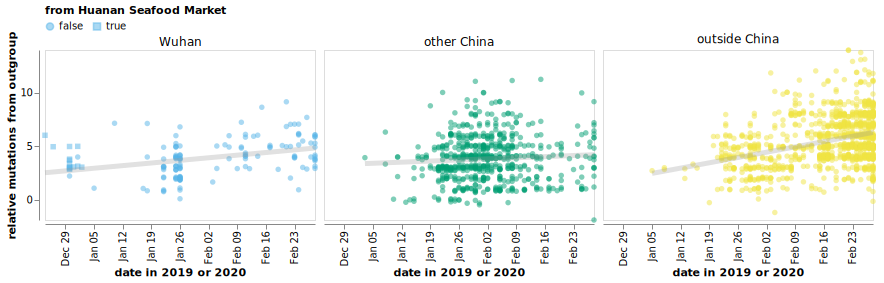
\includegraphics[width=\linewidth]{figures/deltadist_RpYN06.pdf}}
{\bf \LARGE B} \\
\centerline{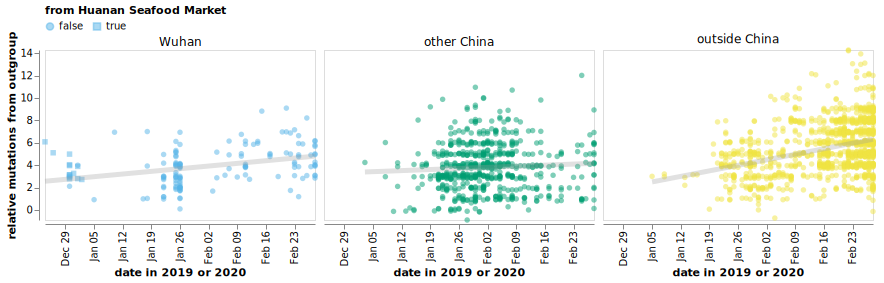
\includegraphics[width=\linewidth]{figures/deltadist_RmYN02.pdf}}
\caption{Versions of Figure~\ref{fig:deltadist_RaTG13} but calculating the relative mutational distances using an outgroup of (A) RpYN06 or (B) RmYN02.
}
\label{suppfig:deltadist_RpYN06_RmYN02}
\end{figure}

 \begin{figure}[h!]
 \centerline{
 \includegraphics[width=0.31\linewidth, valign=t, clip=true, trim=0in 4.4in 0in 0in]{figures/tree_images/hCoV-19-USA-WA1-2020_RpYN06_without_deleted_seqs.pdf}
 \hspace{0.04\linewidth}
 \includegraphics[width=0.32\linewidth, valign=t, clip=true]{figures/tree_images/hCoV-19-Guangdong-HKU-SZ-002-2020_RpYN06_without_deleted_seqs.pdf}
  \hspace{0.04\linewidth}
 \includegraphics[width=0.31\linewidth, valign=t, clip=true, trim=0in 4.4in 0in 0in]{figures/tree_images/hCoV-19-Shandong-LY005-2-2020_RpYN06_without_deleted_seqs.pdf}
 }
 \caption{
 A version of Figure~\ref{fig:tree_RaTG13} but rooting using an outgroup of RpYN06.
 The tree topologies are identical to those obtained using RaTG13 in Figure~\ref{fig:tree_RaTG13}, with the only differences being a few minor changes in which mutations on branches are towards the outgroup (purple mutation labels).
\label{suppfig:tree_RpYN06}
 }
 \end{figure}
 
  \begin{figure}[h!]
\centerline{
 \includegraphics[width=0.31\linewidth, valign=t, clip=true, trim=0in 4.4in 0in 0in]{figures/tree_images/hCoV-19-USA-WA1-2020_RmYN02_without_deleted_seqs.pdf}
 \hspace{0.04\linewidth}
 \includegraphics[width=0.32\linewidth, valign=t, clip=true, trim=0in 4.4in 0in 0in]{figures/tree_images/hCoV-19-Guangdong-HKU-SZ-002-2020_RmYN02_without_deleted_seqs.pdf}
  \hspace{0.04\linewidth}
 \includegraphics[width=0.31\linewidth, valign=t, clip=true, trim=0in 4.4in 0in 0in]{figures/tree_images/hCoV-19-Shandong-LY005-2-2020_RmYN02_without_deleted_seqs.pdf}
 }
 \caption{
 A version of Figure~\ref{fig:tree_RaTG13} but rooting using an outgroup of RmYN02 outgroups.
 The tree topologies are identical to those obtained using RaTG13 in Figure~\ref{fig:tree_RaTG13}, with the only differences being a few minor changes in which mutations on branches are towards the outgroup (purple mutation labels).
\label{suppfig:tree_RmYN02}
 }
 \end{figure}




\end{document}
